\documentclass{standalone}
\usepackage{tikz}
\usetikzlibrary{patterns, positioning}


\begin{document}
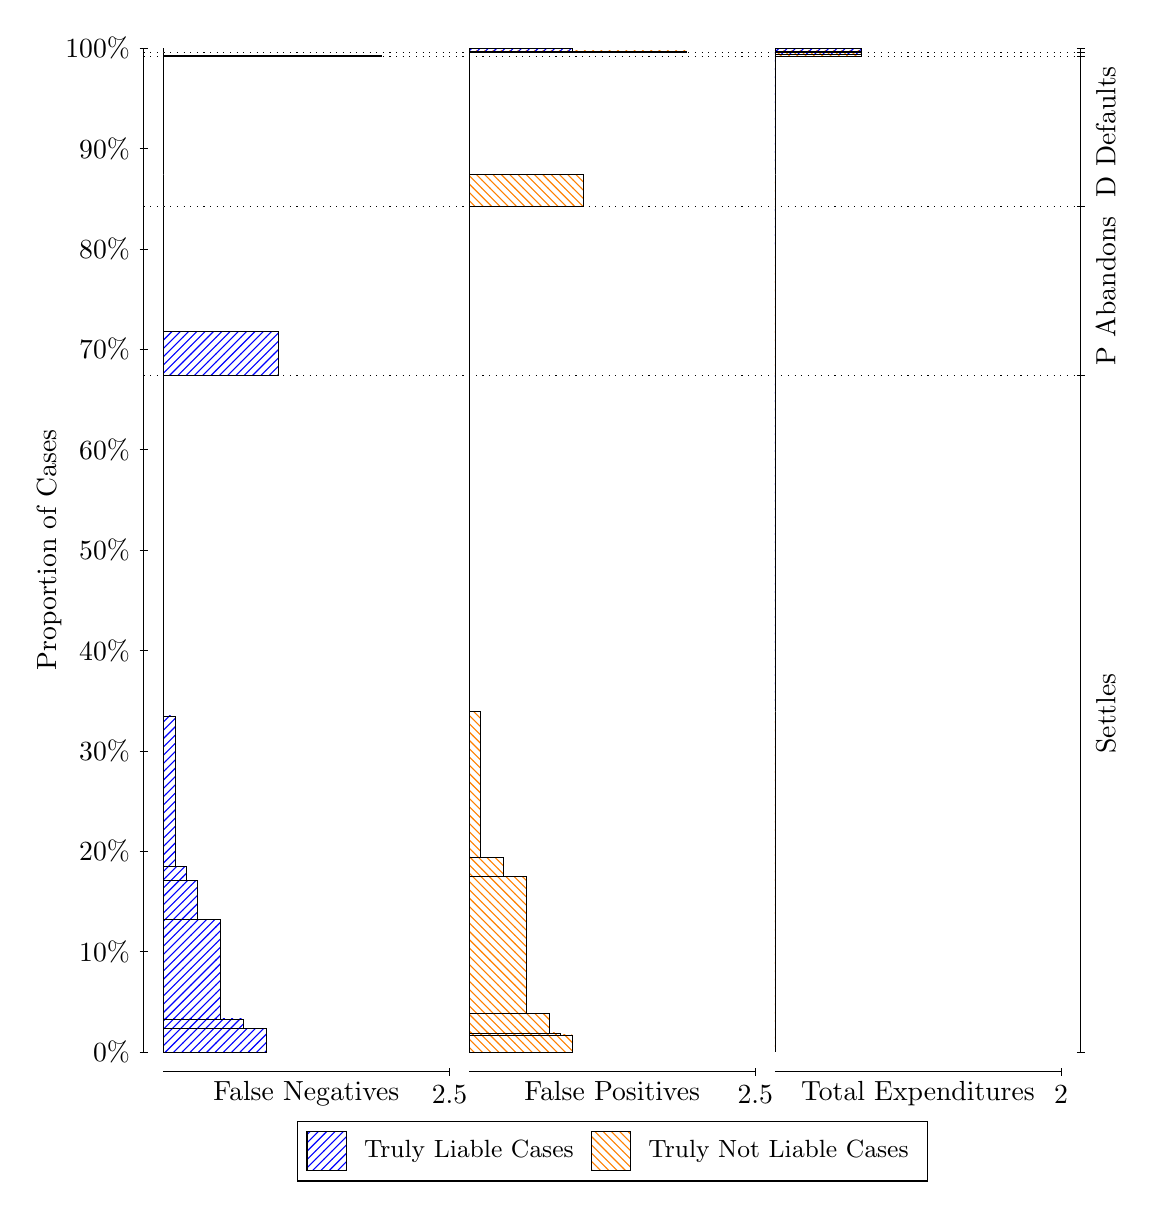
\begin{tikzpicture}
\draw[black, very thin] (1.5,1.75) -- (1.5,14.5);
\node[rotate=90, text=black, anchor=center] at (0.3, 8.125) {Proportion of Cases};
\draw[black, very thin] (1.45,1.75) -- (1.55,1.75);
\node[text=black, anchor=east] at (1.45, 1.75) {0\%};
\draw[black, very thin] (1.45,3.025) -- (1.55,3.025);
\node[text=black, anchor=east] at (1.45, 3.025) {10\%};
\draw[black, very thin] (1.45,4.3) -- (1.55,4.3);
\node[text=black, anchor=east] at (1.45, 4.3) {20\%};
\draw[black, very thin] (1.45,5.575) -- (1.55,5.575);
\node[text=black, anchor=east] at (1.45, 5.575) {30\%};
\draw[black, very thin] (1.45,6.85) -- (1.55,6.85);
\node[text=black, anchor=east] at (1.45, 6.85) {40\%};
\draw[black, very thin] (1.45,8.125) -- (1.55,8.125);
\node[text=black, anchor=east] at (1.45, 8.125) {50\%};
\draw[black, very thin] (1.45,9.4) -- (1.55,9.4);
\node[text=black, anchor=east] at (1.45, 9.4) {60\%};
\draw[black, very thin] (1.45,10.675) -- (1.55,10.675);
\node[text=black, anchor=east] at (1.45, 10.675) {70\%};
\draw[black, very thin] (1.45,11.95) -- (1.55,11.95);
\node[text=black, anchor=east] at (1.45, 11.95) {80\%};
\draw[black, very thin] (1.45,13.225) -- (1.55,13.225);
\node[text=black, anchor=east] at (1.45, 13.225) {90\%};
\draw[black, very thin] (1.45,14.5) -- (1.55,14.5);
\node[text=black, anchor=east] at (1.45, 14.5) {100\%};

\draw[black, very thin] (13.4,1.75) -- (13.4,14.5);
\draw[black, very thin] (13.35,1.75) -- (13.45,1.75);
\node[anchor=west] at (13.35, 1.75) {};
\draw[black, very thin] (13.35,10.346) -- (13.45,10.346);
\node[anchor=west] at (13.35, 10.346) {};
\draw[black, very thin] (13.35,12.486) -- (13.45,12.486);
\node[anchor=west] at (13.35, 12.486) {};
\draw[black, very thin] (13.35,14.389) -- (13.45,14.389);
\node[anchor=west] at (13.35, 14.389) {};
\draw[black, very thin] (13.35,14.445) -- (13.45,14.445);
\node[anchor=west] at (13.35, 14.445) {};
\draw[black, very thin] (13.35,14.5) -- (13.45,14.5);
\node[anchor=west] at (13.35, 14.5) {};

\draw[black, very thin, pattern color=blue, pattern=north east lines] (1.75,1.75) rectangle (3.058,2.0476);
\draw[black, very thin, pattern color=blue, pattern=north east lines] (1.75,2.0476) rectangle (2.7673,2.169);
\draw[black, very thin, pattern color=blue, pattern=north east lines] (1.75,2.169) rectangle (2.622,2.1709);
\draw[black, very thin, pattern color=blue, pattern=north east lines] (1.75,2.1709) rectangle (2.4767,3.436);
\draw[black, very thin, pattern color=blue, pattern=north east lines] (1.75,3.436) rectangle (2.186,3.9276);
\draw[black, very thin, pattern color=blue, pattern=north east lines] (1.75,3.9276) rectangle (2.0407,4.1077);
\draw[black, very thin, pattern color=blue, pattern=north east lines] (1.75,4.1077) rectangle (1.8953,6.0195);
\draw[black, very thin, pattern color=orange, pattern=north west lines] (1.75,6.0195) rectangle (1.75,10.346);
\draw[black, very thin, pattern color=blue, pattern=north east lines] (1.75,10.346) rectangle (3.2033,10.9);
\draw[black, very thin, pattern color=orange, pattern=north west lines] (1.75,10.9) rectangle (1.75,12.486);
\draw[black, very thin, pattern color=orange, pattern=north west lines] (1.75,12.486) rectangle (1.75,12.893);
\draw[black, very thin, pattern color=blue, pattern=north east lines] (1.75,12.893) rectangle (1.75,14.389);
\draw[black, very thin, pattern color=blue, pattern=north east lines] (1.75,14.389) rectangle (4.5113,14.408);
\draw[black, very thin, pattern color=orange, pattern=north west lines] (1.75,14.408) rectangle (1.75,14.445);
\draw[black, very thin, pattern color=orange, pattern=north west lines] (1.75,14.445) rectangle (1.75,14.463);
\draw[black, very thin, pattern color=blue, pattern=north east lines] (1.75,14.463) rectangle (1.75,14.5);
\draw[black, very thin, pattern color=orange, pattern=north west lines] (5.6333,1.75) rectangle (6.9413,1.9657);
\draw[black, very thin, pattern color=orange, pattern=north west lines] (5.6333,1.9657) rectangle (6.796,1.9919);
\draw[black, very thin, pattern color=orange, pattern=north west lines] (5.6333,1.9919) rectangle (6.6507,2.2378);
\draw[black, very thin, pattern color=orange, pattern=north west lines] (5.6333,2.2378) rectangle (6.36,3.9825);
\draw[black, very thin, pattern color=orange, pattern=north west lines] (5.6333,3.9825) rectangle (6.2147,3.9835);
\draw[black, very thin, pattern color=orange, pattern=north west lines] (5.6333,3.9835) rectangle (6.0693,4.219);
\draw[black, very thin, pattern color=orange, pattern=north west lines] (5.6333,4.219) rectangle (5.7787,6.077);
\draw[black, very thin, pattern color=blue, pattern=north east lines] (5.6333,6.077) rectangle (5.6333,10.346);
\draw[black, very thin, pattern color=orange, pattern=north west lines] (5.6333,10.346) rectangle (5.6333,11.933);
\draw[black, very thin, pattern color=blue, pattern=north east lines] (5.6333,11.933) rectangle (5.6333,12.486);
\draw[black, very thin, pattern color=orange, pattern=north west lines] (5.6333,12.486) rectangle (7.0867,12.893);
\draw[black, very thin, pattern color=blue, pattern=north east lines] (5.6333,12.893) rectangle (5.6333,14.389);
\draw[black, very thin, pattern color=orange, pattern=north west lines] (5.6333,14.389) rectangle (5.6333,14.426);
\draw[black, very thin, pattern color=blue, pattern=north east lines] (5.6333,14.426) rectangle (5.6333,14.445);
\draw[black, very thin, pattern color=orange, pattern=north west lines] (5.6333,14.445) rectangle (8.3947,14.463);
\draw[black, very thin, pattern color=blue, pattern=north east lines] (5.6333,14.463) rectangle (6.9413,14.5);
\draw[black, very thin, pattern color=orange, pattern=north west lines] (9.5167,1.75) rectangle (9.5167,6.077);
\draw[black, very thin, pattern color=blue, pattern=north east lines] (9.5167,6.077) rectangle (9.5167,10.346);
\draw[black, very thin, pattern color=orange, pattern=north west lines] (9.5167,10.346) rectangle (9.5167,11.933);
\draw[black, very thin, pattern color=blue, pattern=north east lines] (9.5167,11.933) rectangle (9.5167,12.486);
\draw[black, very thin, pattern color=orange, pattern=north west lines] (9.5167,12.486) rectangle (9.5167,12.893);
\draw[black, very thin, pattern color=blue, pattern=north east lines] (9.5167,12.893) rectangle (9.5167,14.389);
\draw[black, very thin, pattern color=orange, pattern=north west lines] (9.5167,14.389) rectangle (10.607,14.426);
\draw[black, very thin, pattern color=blue, pattern=north east lines] (9.5167,14.426) rectangle (10.607,14.445);
\draw[black, very thin, pattern color=orange, pattern=north west lines] (9.5167,14.445) rectangle (10.607,14.463);
\draw[black, very thin, pattern color=blue, pattern=north east lines] (9.5167,14.463) rectangle (10.607,14.5);
\draw[black, dotted] (1.5,10.346) -- (13.4,10.346);
\draw[black, dotted] (1.5,12.486) -- (13.4,12.486);
\draw[black, dotted] (1.5,14.389) -- (13.4,14.389);
\draw[black, dotted] (1.5,14.445) -- (13.4,14.445);
\draw[black, very thin] (1.75,1.5) -- (5.3833,1.5);
\node[text=black, anchor=north] at (3.5667, 1.5) {False Negatives};
\draw[black, very thin] (5.3833,1.45) -- (5.3833,1.55);
\node[text=black, anchor=north] at (5.3833, 1.45) {2.5};

\draw[black, very thin] (5.6333,1.5) -- (9.2667,1.5);
\node[text=black, anchor=north] at (7.45, 1.5) {False Positives};
\draw[black, very thin] (9.2667,1.45) -- (9.2667,1.55);
\node[text=black, anchor=north] at (9.2667, 1.45) {2.5};

\draw[black, very thin] (9.5167,1.5) -- (13.15,1.5);
\node[text=black, anchor=north] at (11.333, 1.5) {Total Expenditures};
\draw[black, very thin] (13.15,1.45) -- (13.15,1.55);
\node[text=black, anchor=north] at (13.15, 1.45) {2};

\node[text=black, centered, rotate=90] at (13.72, 6.0482) {Settles};
\node[text=black, centered, rotate=90] at (13.72, 11.416) {P Abandons};
\node[text=black, centered, rotate=90] at (13.72, 13.438) {D Defaults};



\draw (7.449999999999999,1.5) node[draw=none] (baseCoordinate) {};
\begin{scope}[align=center]
        \matrix[scale=0.5, draw=black, below=0.5cm of baseCoordinate, nodes={draw}, column sep=0.1cm]{
            \node[rectangle, draw, minimum width=0.5cm, minimum height=0.5cm, pattern color=blue, pattern=north east lines] {}; &
            \node[draw=none, font=\small, text=black] (B) {Truly Liable Cases}; &
            \node[rectangle, draw, minimum width=0.5cm, minimum height=0.5cm, pattern color=orange, pattern=north west lines] {}; &
            \node[draw=none, font=\small, text=black] (B) {Truly Not Liable Cases}; \\
            };
\end{scope}

\end{tikzpicture}
\end{document}